
\documentclass{beamer}

\usepackage{algpseudocode, color, colortbl, listings, MnSymbol}

\usepackage{hyperref}
\hypersetup{
    colorlinks=true,
    urlcolor=blue,
}

\usetheme{Montpellier}
\usecolortheme{rose}

% page numbers, from
% https://tex.stackexchange.com/questions/137022/how-to-insert-page-number-in-beamer-navigation-symbols
\expandafter\def\expandafter\insertshorttitle\expandafter{%
  \insertshorttitle\hfill%
  \insertframenumber\,/\,\inserttotalframenumber}

\definecolor{Gray}{gray}{0.8}
\newcolumntype{g}{>{\columncolor{Gray}}c}

\newcommand{\stanza}{ \\~\ }

\title{18. Approximate TSP}
\subtitle{CPSC 535}
\author{Kevin A. Wortman}
\institute{ 
\includegraphics[height=2cm]{csuf-logo-cmyk} }
\date{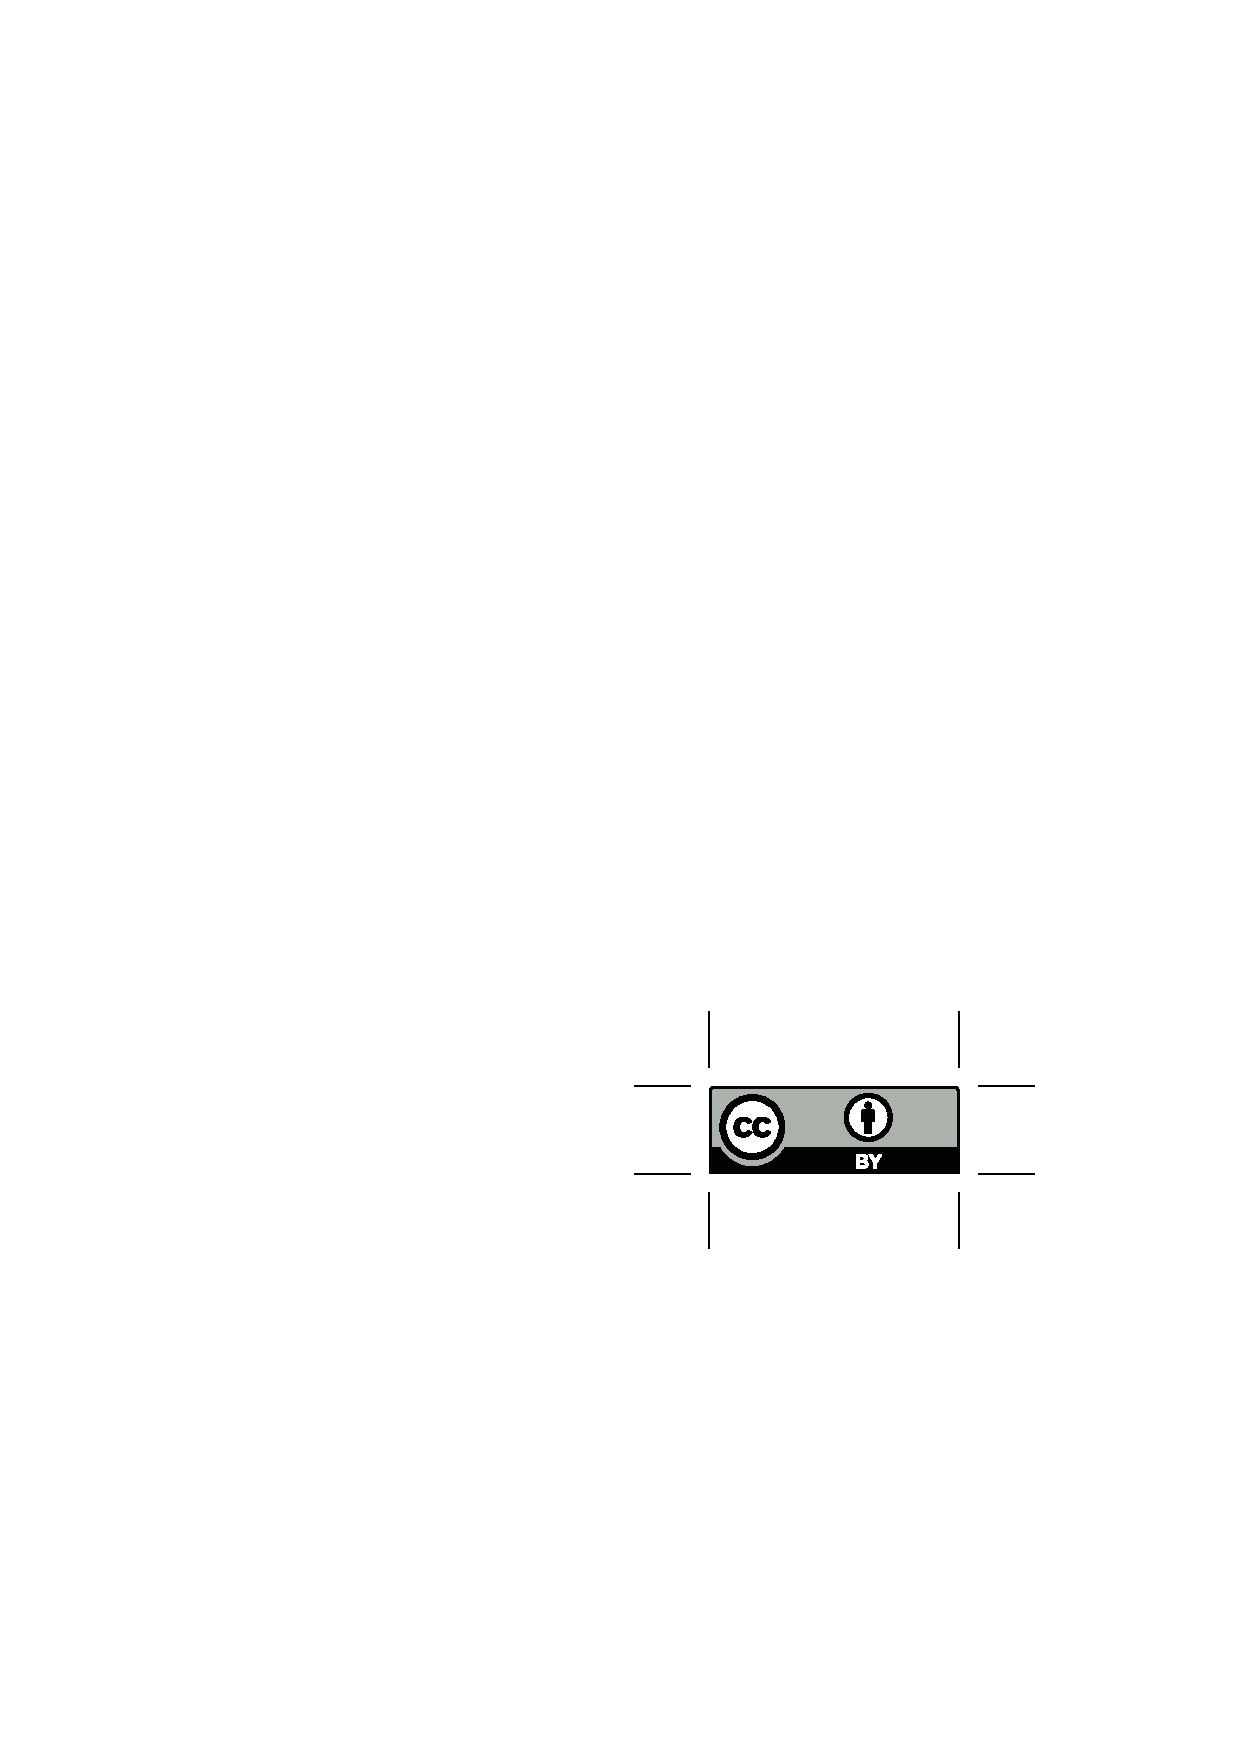
\includegraphics[height=14pt]{by} \\

{\tiny
This work is licensed under a
\href{http://creativecommons.org/licenses/by/4.0/}{Creative Commons Attribution 4.0 International License}.
}}

\begin{document}

\begin{frame}
  \titlepage
\end{frame}

\begin{frame} \frametitle{TSP}
\emph{traveling salesperson problem (TSP)} \\
\textbf{input}: a complete undirected graph $G=(V,E)$ where each edge has weight $w(e) \geq 0$ \\
\textbf{output}: a sequence of vertices $H$ forming a Hamiltonian cycle, minimizing
total edge weight
\stanza

Recall:
\begin{itemize}
  \item \emph{Cycle:} path that starts and ends at same vertex
  \item \emph{Hamiltonian:} visits each vertex exactly once
  \item every complete graph contains some Hamiltonian cycle
\end{itemize}

\textbf{Bad news:}
\begin{itemize}
  \item TSP is $NP$-complete; if $P \ne NP$, no polynomial-time optimization algorithm
  \item TSP is also $APX$-complete; if $P \ne NP,$ no PTAS
\end{itemize}
\end{frame}

\begin{frame} \frametitle{TSP}
  \begin{center}
    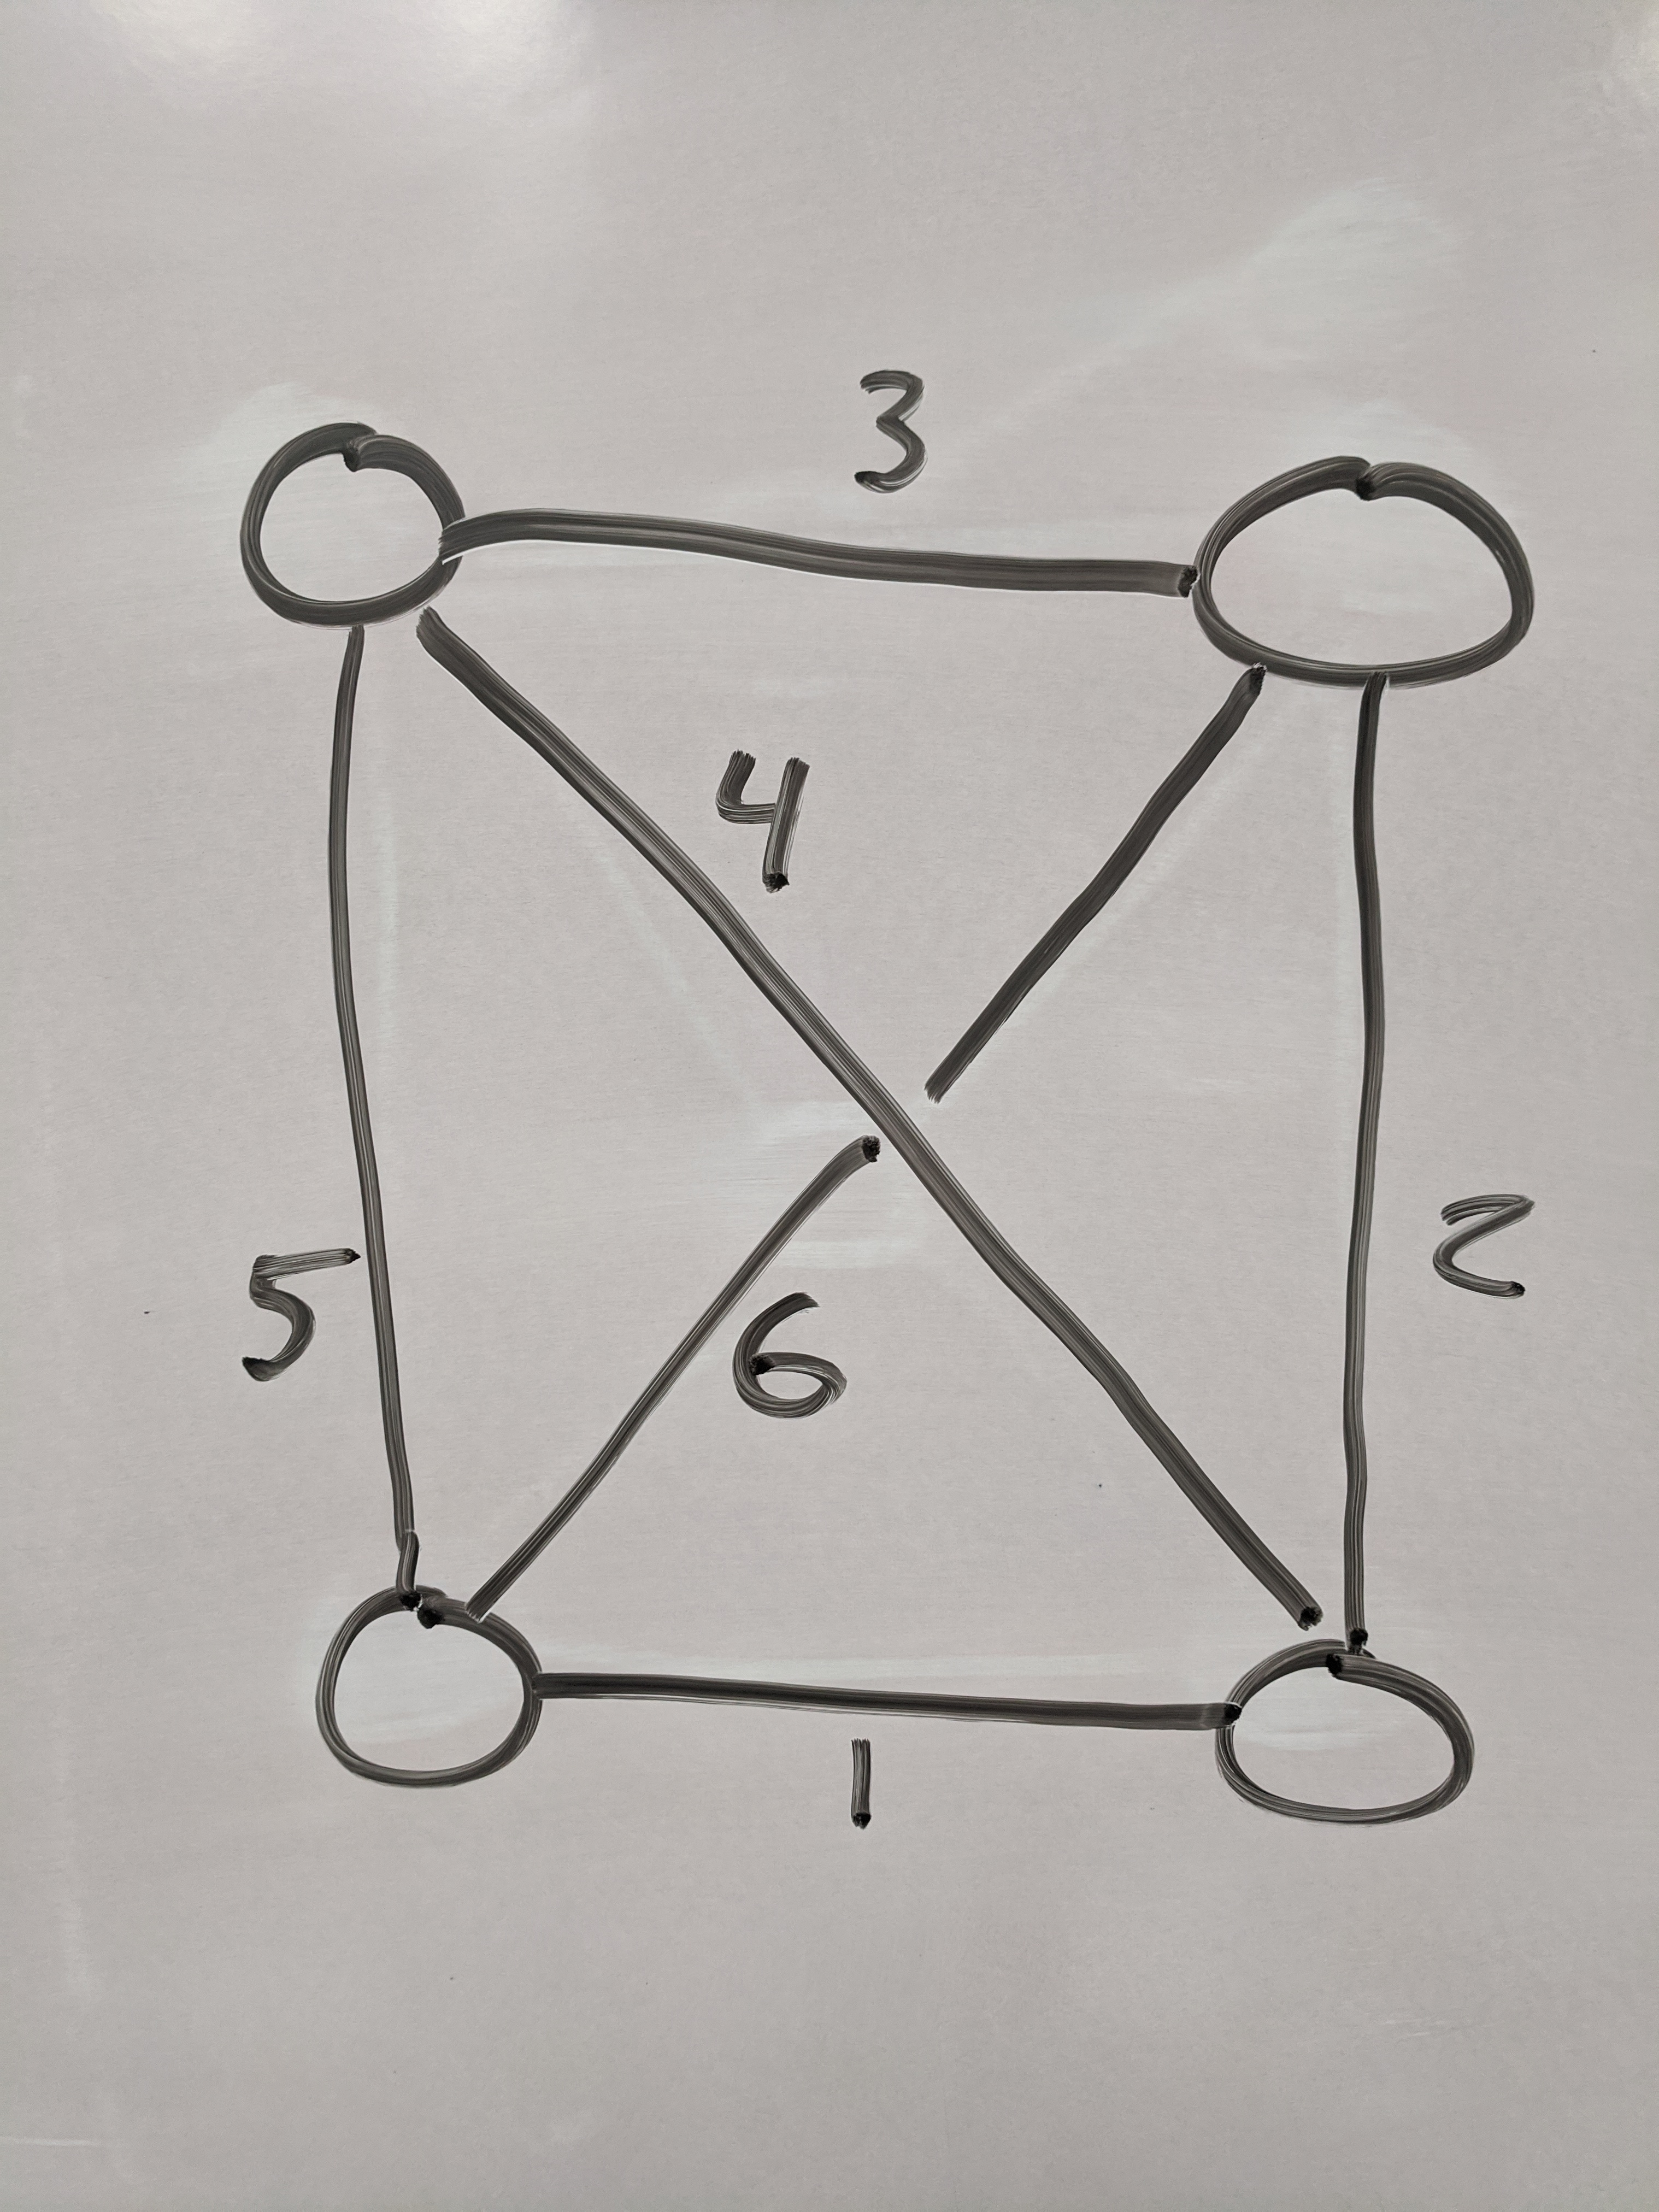
\includegraphics[height=120pt]{13-tsp-input.jpg}
    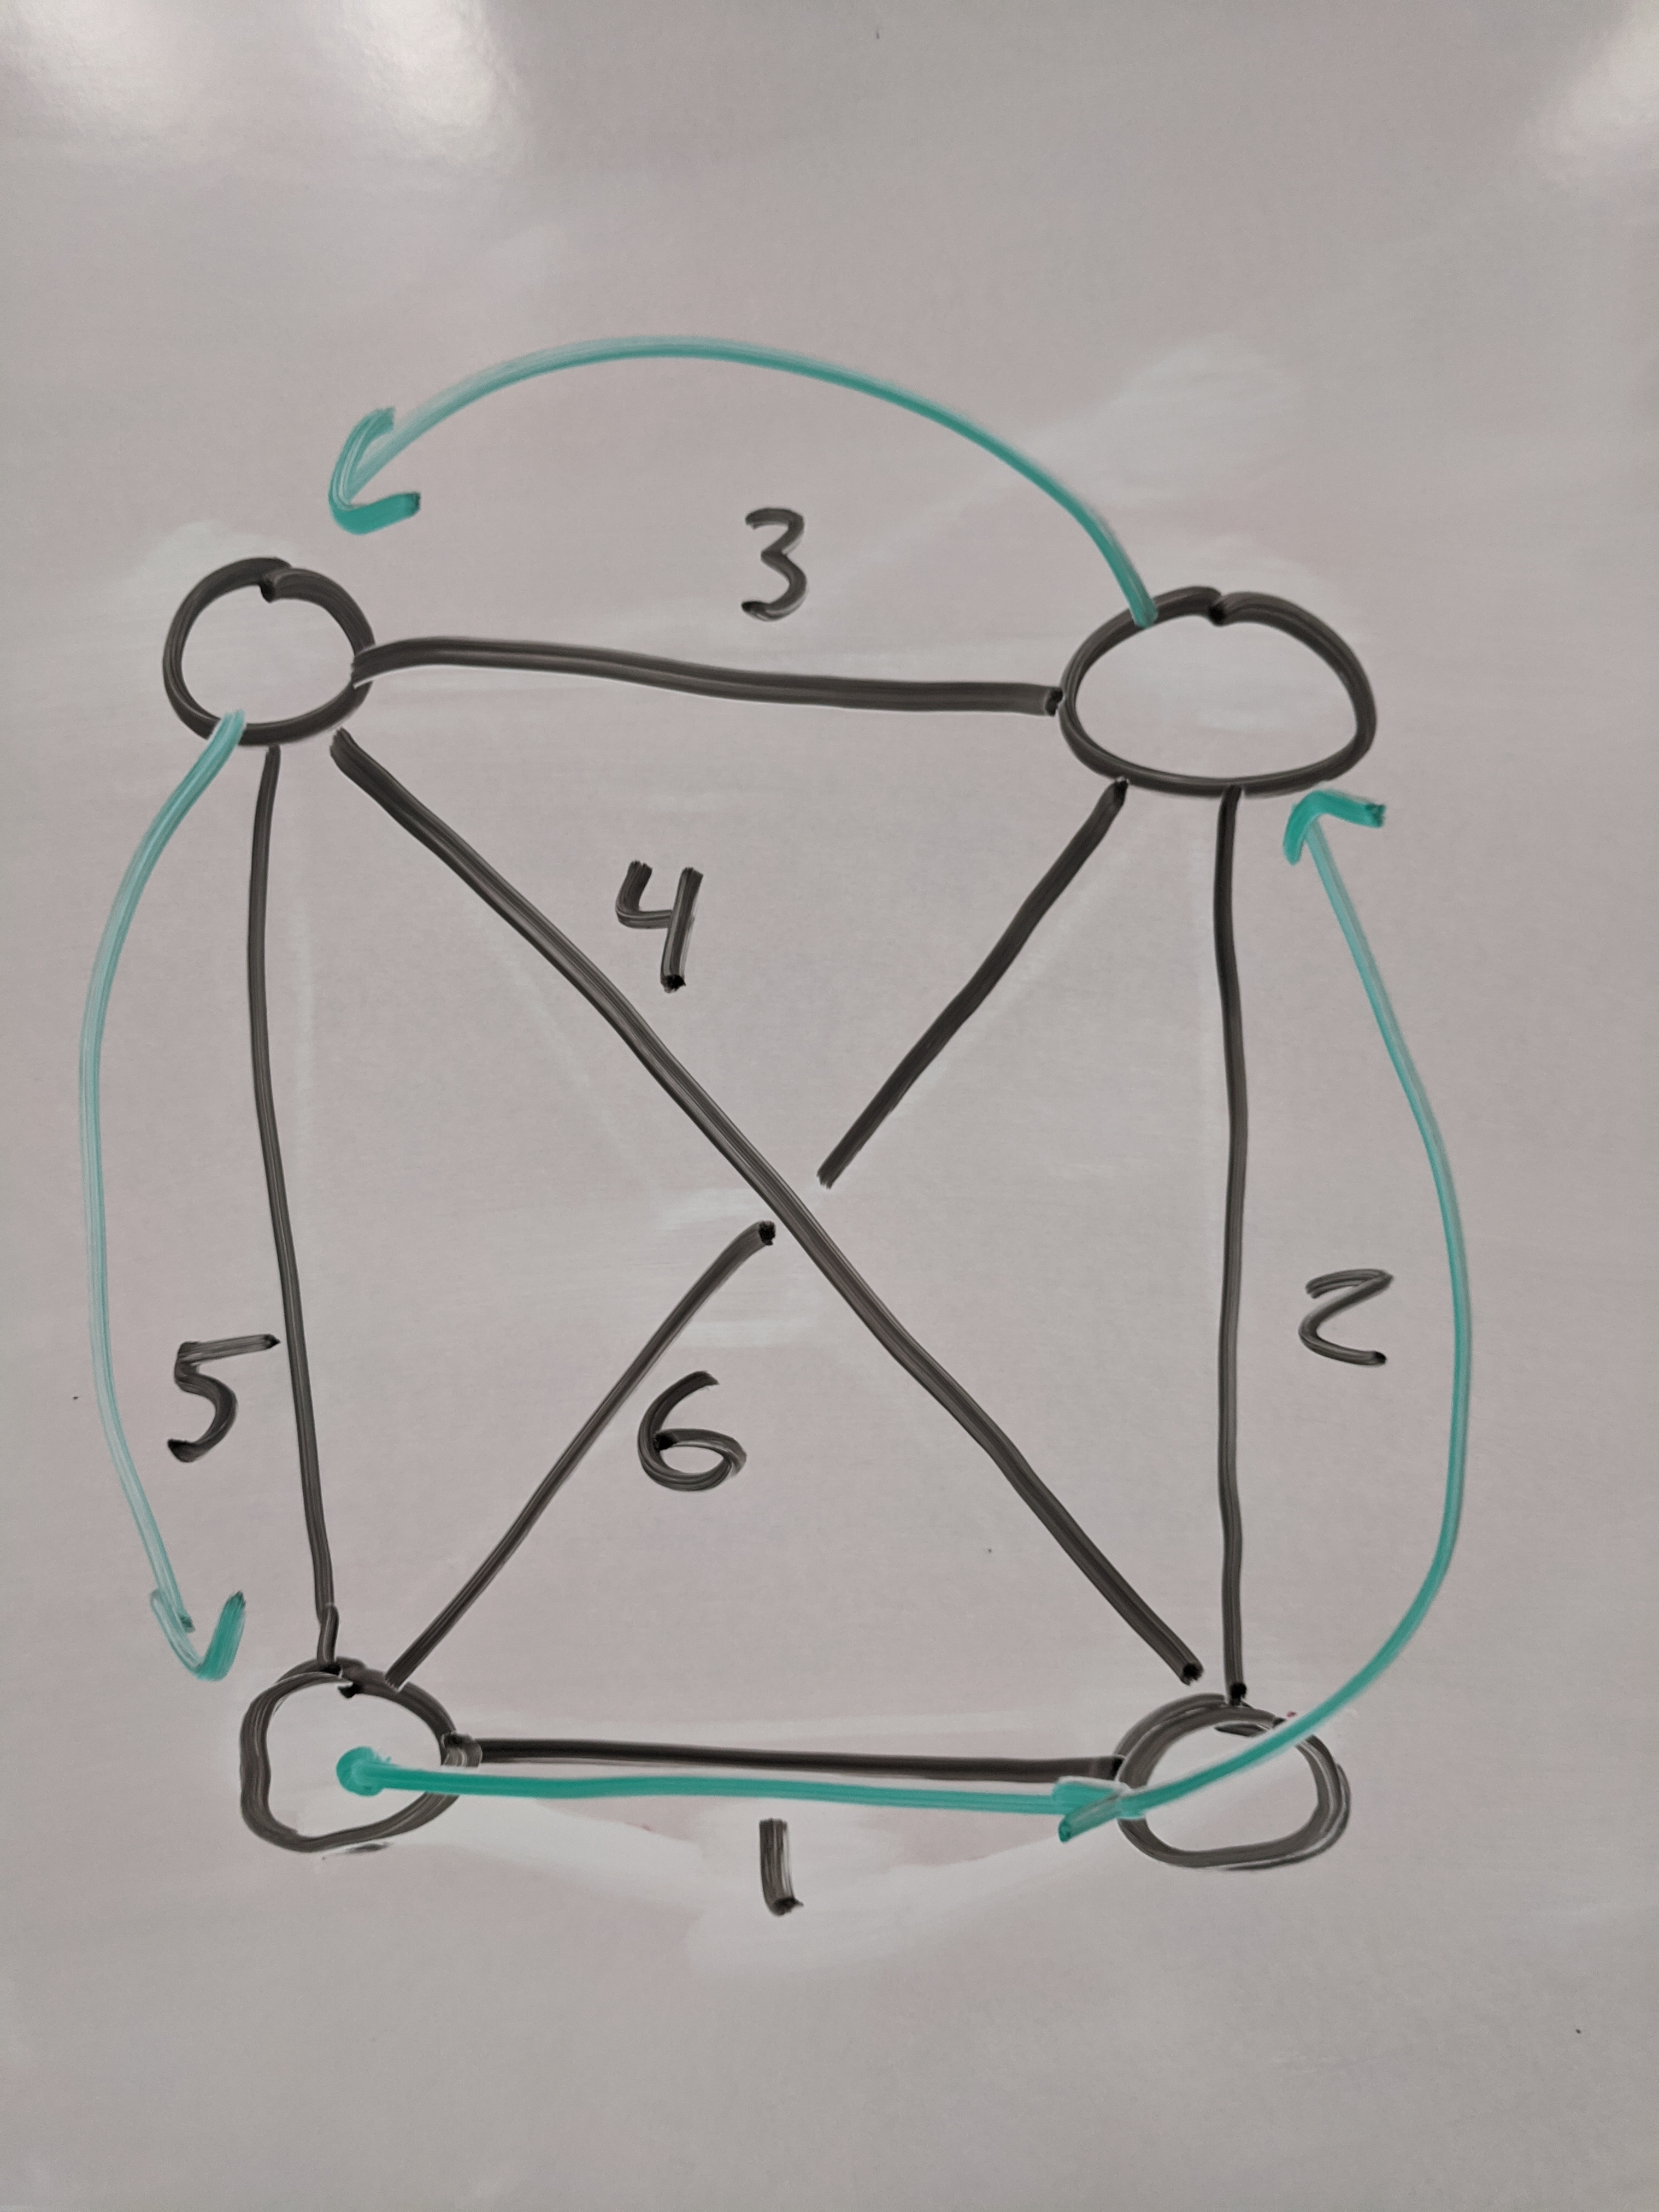
\includegraphics[height=120pt]{13-tsp-output.jpg}
  \end{center}
\end{frame}

\begin{frame} \frametitle{Triangle Inequality}
Triangle inequality in general: for distance function $d$ and sites $a, b, c,$
\[ d(a, c) \leq d(a, b) + d(b, c) \]
$\Rightarrow$ direct path $a \rightarrow c$ always cheaper than two-step path
$a \rightarrow b \rightarrow c$ (or tied) \stanza

Triangle inequality in a complete graph: for vertices $x, y, z$ and edge weights $w,$
\[ w(x, z) \leq w(x, y) + w(y, z) \]
$\Rightarrow$ same intuition; adding an intermediate step is never a shortcut \\
$\Rightarrow$ automatically holds for Euclidean graphs
\end{frame}

\begin{frame} \frametitle{TSP with Triangle Inequality (TSPTI)}

\textbf{input}: a complete undirected graph $G=(V,E)$ where each edge has weight $w(e) \geq 0$;
and for any $x, y, z \in V$, $w(x, z) \leq w(x, y) + w(y, z)$ \\
\textbf{output}: (same as conventional TSP) \stanza
\begin{itemize}
  \item \textbf{renegotiating} TSP
  \item different problem; $NP$-completeness and $APX$-completeness proofs may not apply
  \item less-general problem
  \item probably still relevant to practical applications of TSP
\end{itemize}
\end{frame}

\begin{frame} \frametitle{TSPTI Approximation Algorithm Idea}
\begin{itemize}
  \item need a structure that can lower-bound an optimal cycle $H^\star$ and upper-bound
    our approximate cycle $H$
  \item \emph{minimum spanning tree} features
  \begin{itemize}
    \item minimizes weight of chosen edges
    \item connects all vertices
    \item can be computed fast
  \end{itemize}
  \item but an MST is not a Hamiltonian cycle; MST is acyclic, for one thing
  \item \emph{Euler tour:} cycle around a tree; preorder, inorder, postorder
  \item build an MST; perform preorder traversal; treat that vertex order as Hamiltonian cycle
\end{itemize}
\end{frame}

\begin{frame} \frametitle{Review: Minimum Spanning Trees (MST)}
  \begin{center}
    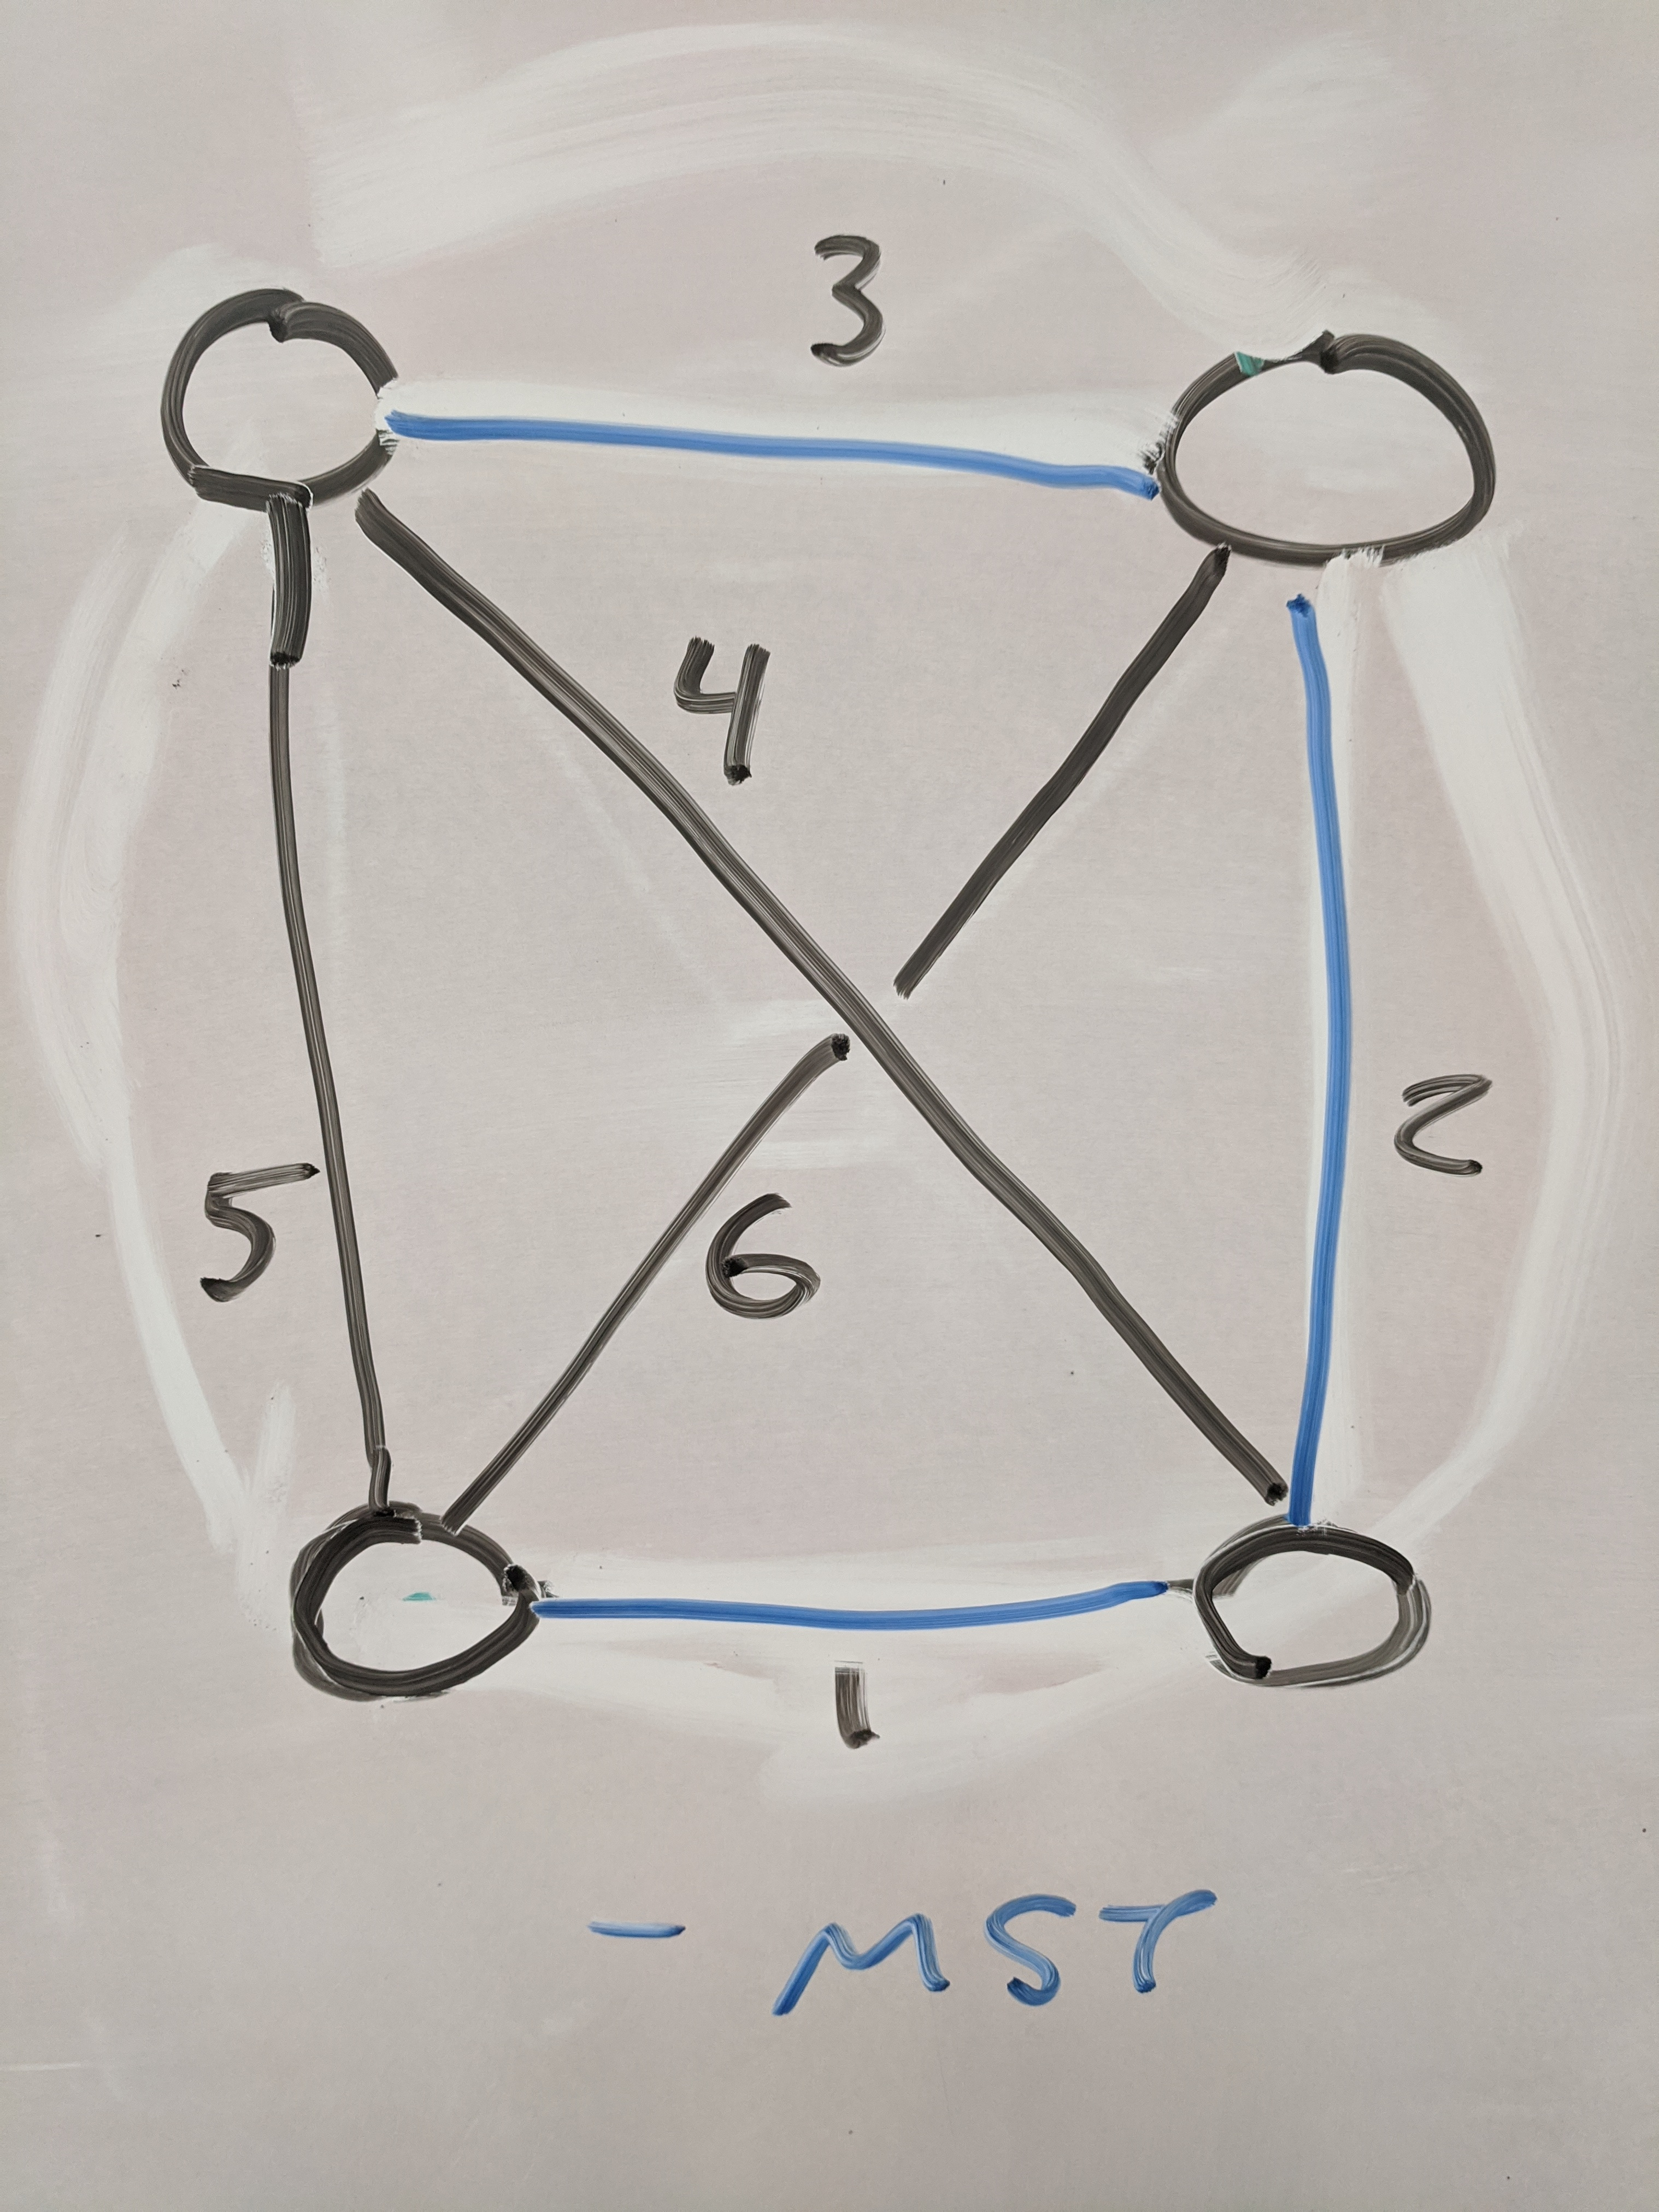
\includegraphics[height=160pt]{13-mst.jpg}
  \end{center}
\end{frame}

\begin{frame} \frametitle{Review: Preorder Traversal}
  \begin{center}
    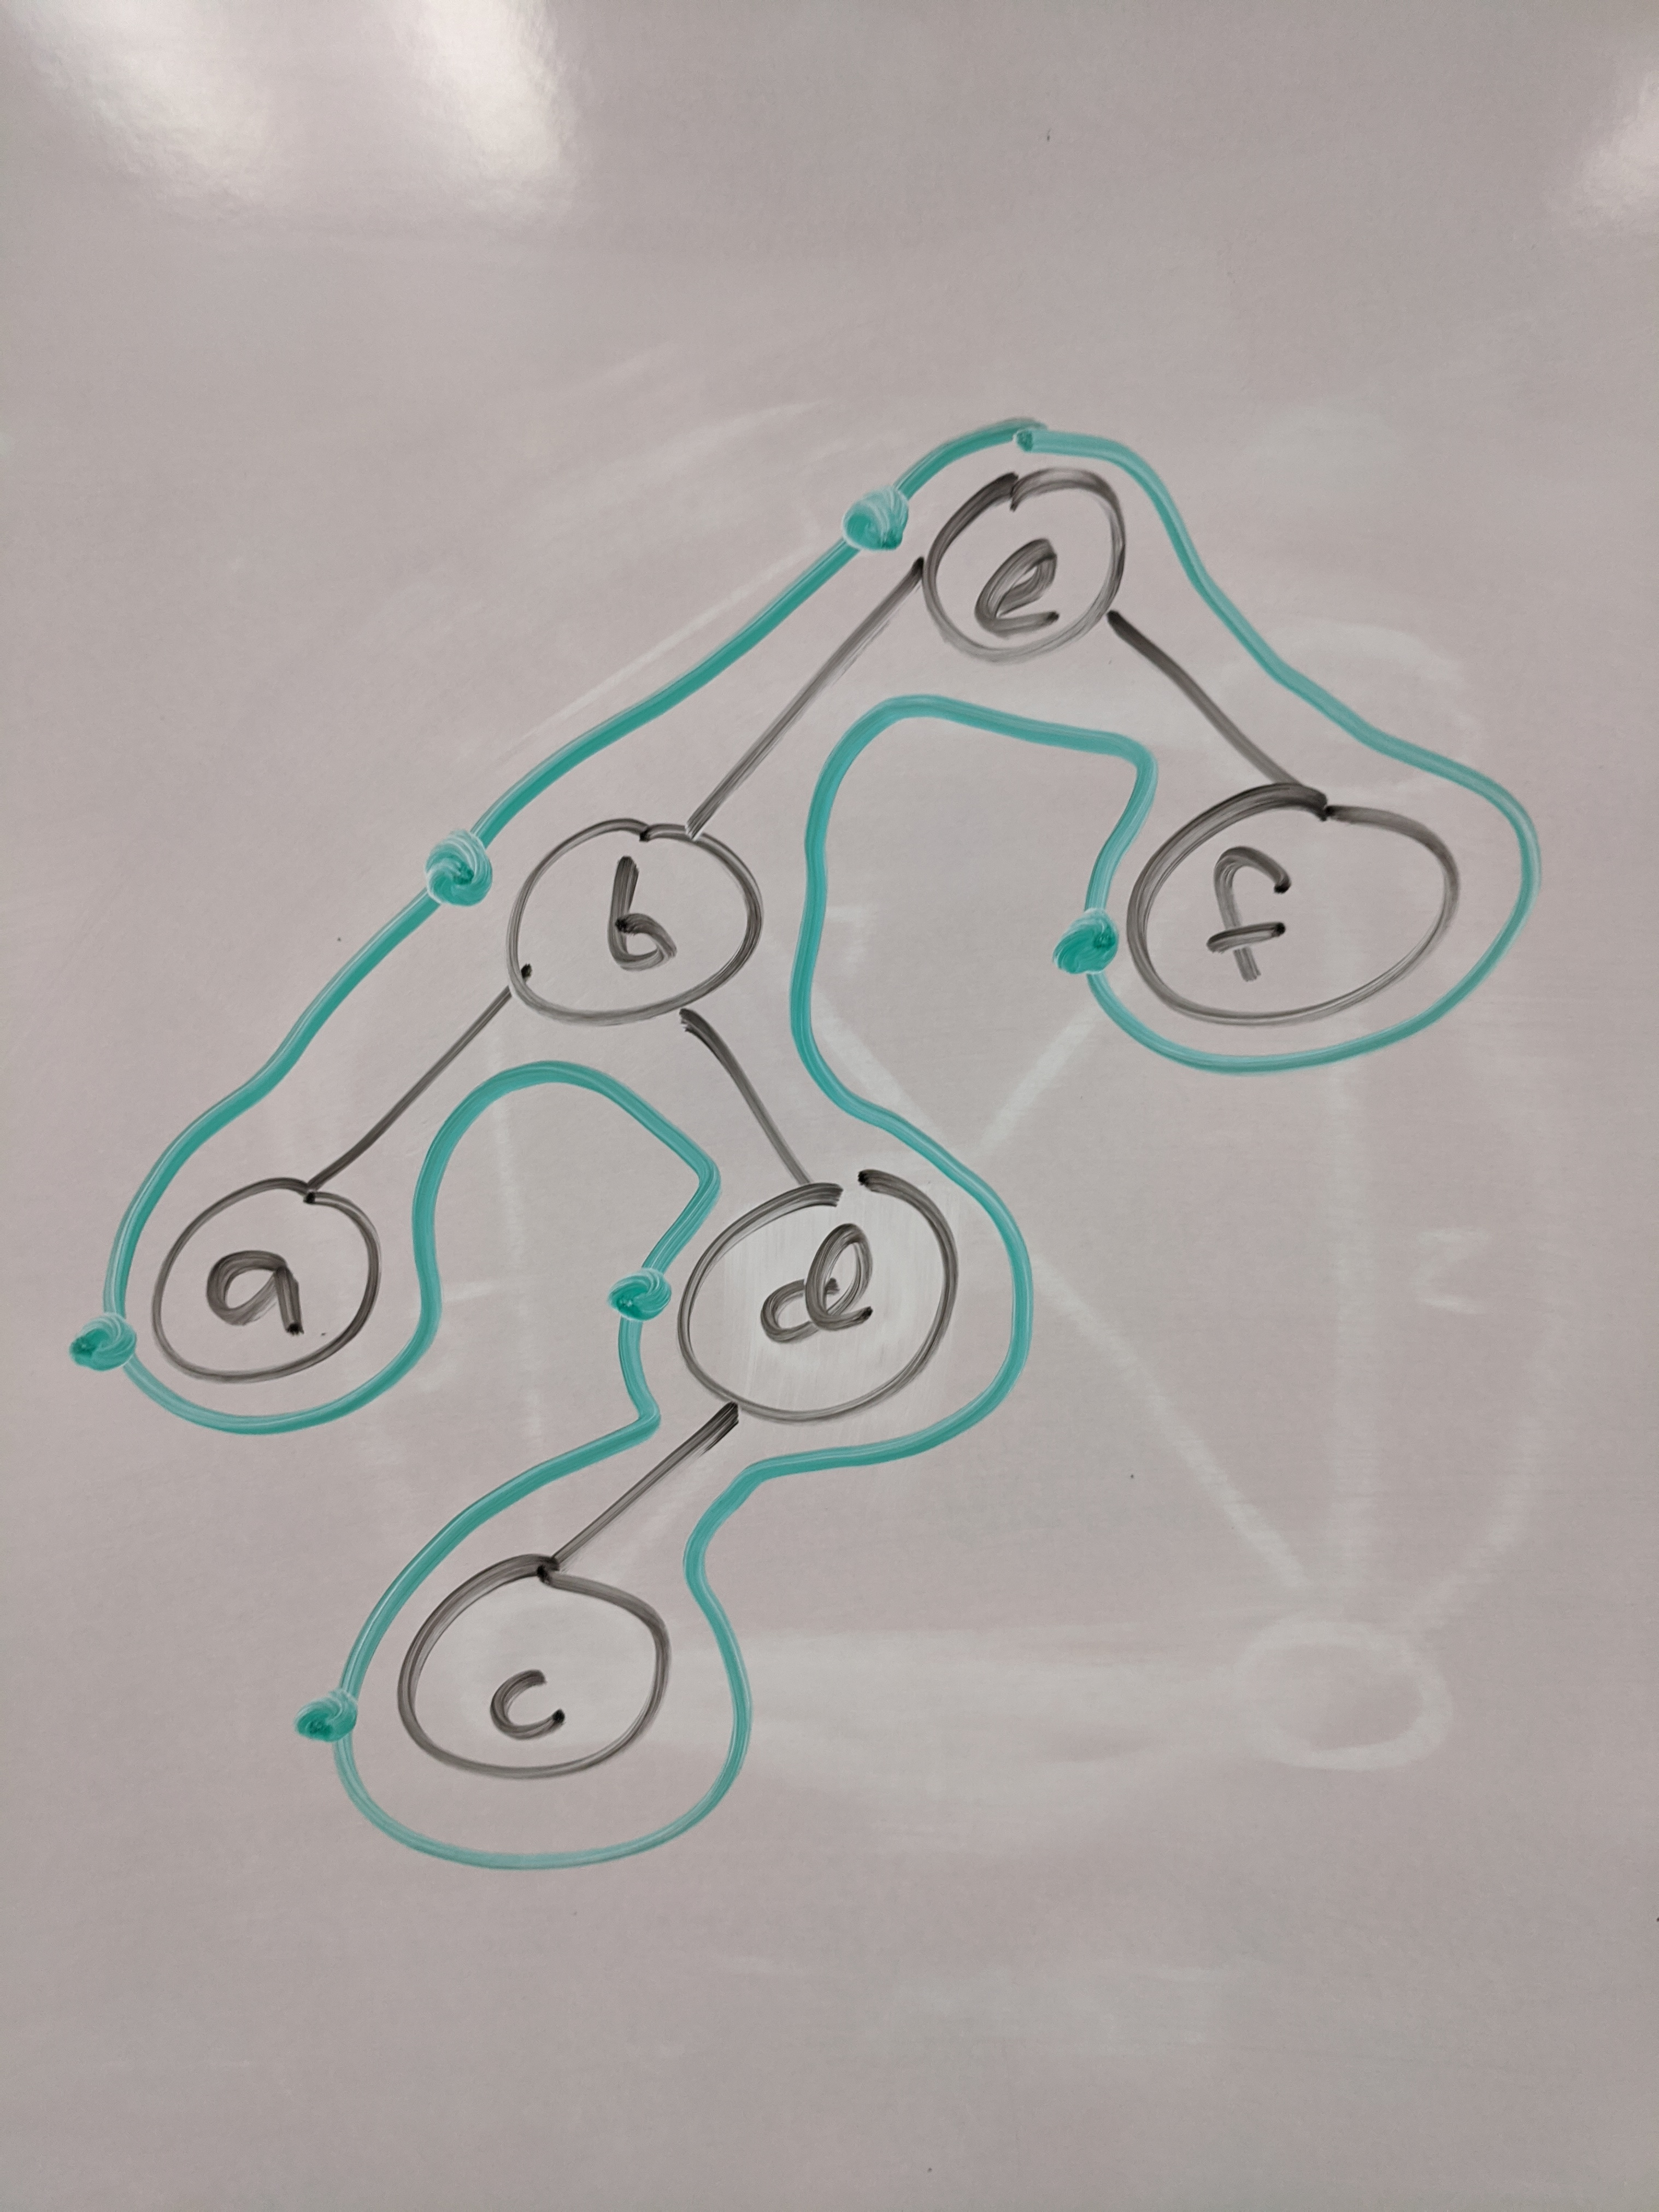
\includegraphics[height=160pt]{13-preorder.jpg}
  \end{center}
\end{frame}

\begin{frame} \frametitle{Approximate TSPTI Pseudocode}
  \begin{algorithmic}[1]
    \Function{APPROX-TSPTI}{$G=(V,E), w$}
      \State $T = PRIM-MST(G, w)$
      \State $H = $ empty sequence of vertices
      \For { vertex $v$ in preorder traversal of tree $T$ }
        \State $H.ADDBACK(v)$
      \EndFor
      \State $H.ADDBACK(H[0])$
      \State \Return $H$
    \EndFunction
  \end{algorithmic}
\vspace{.5 cm}
\textbf{Analysis}: Prim's algorithm takes $O(m + n \log n)$ (w/ Fibonacci heap),
traversal takes $O(m + n)$, total $O(m + n \log n)$ time
\end{frame}

\begin{frame} \frametitle{Approximate TSPTI: MST}
  \begin{center}
    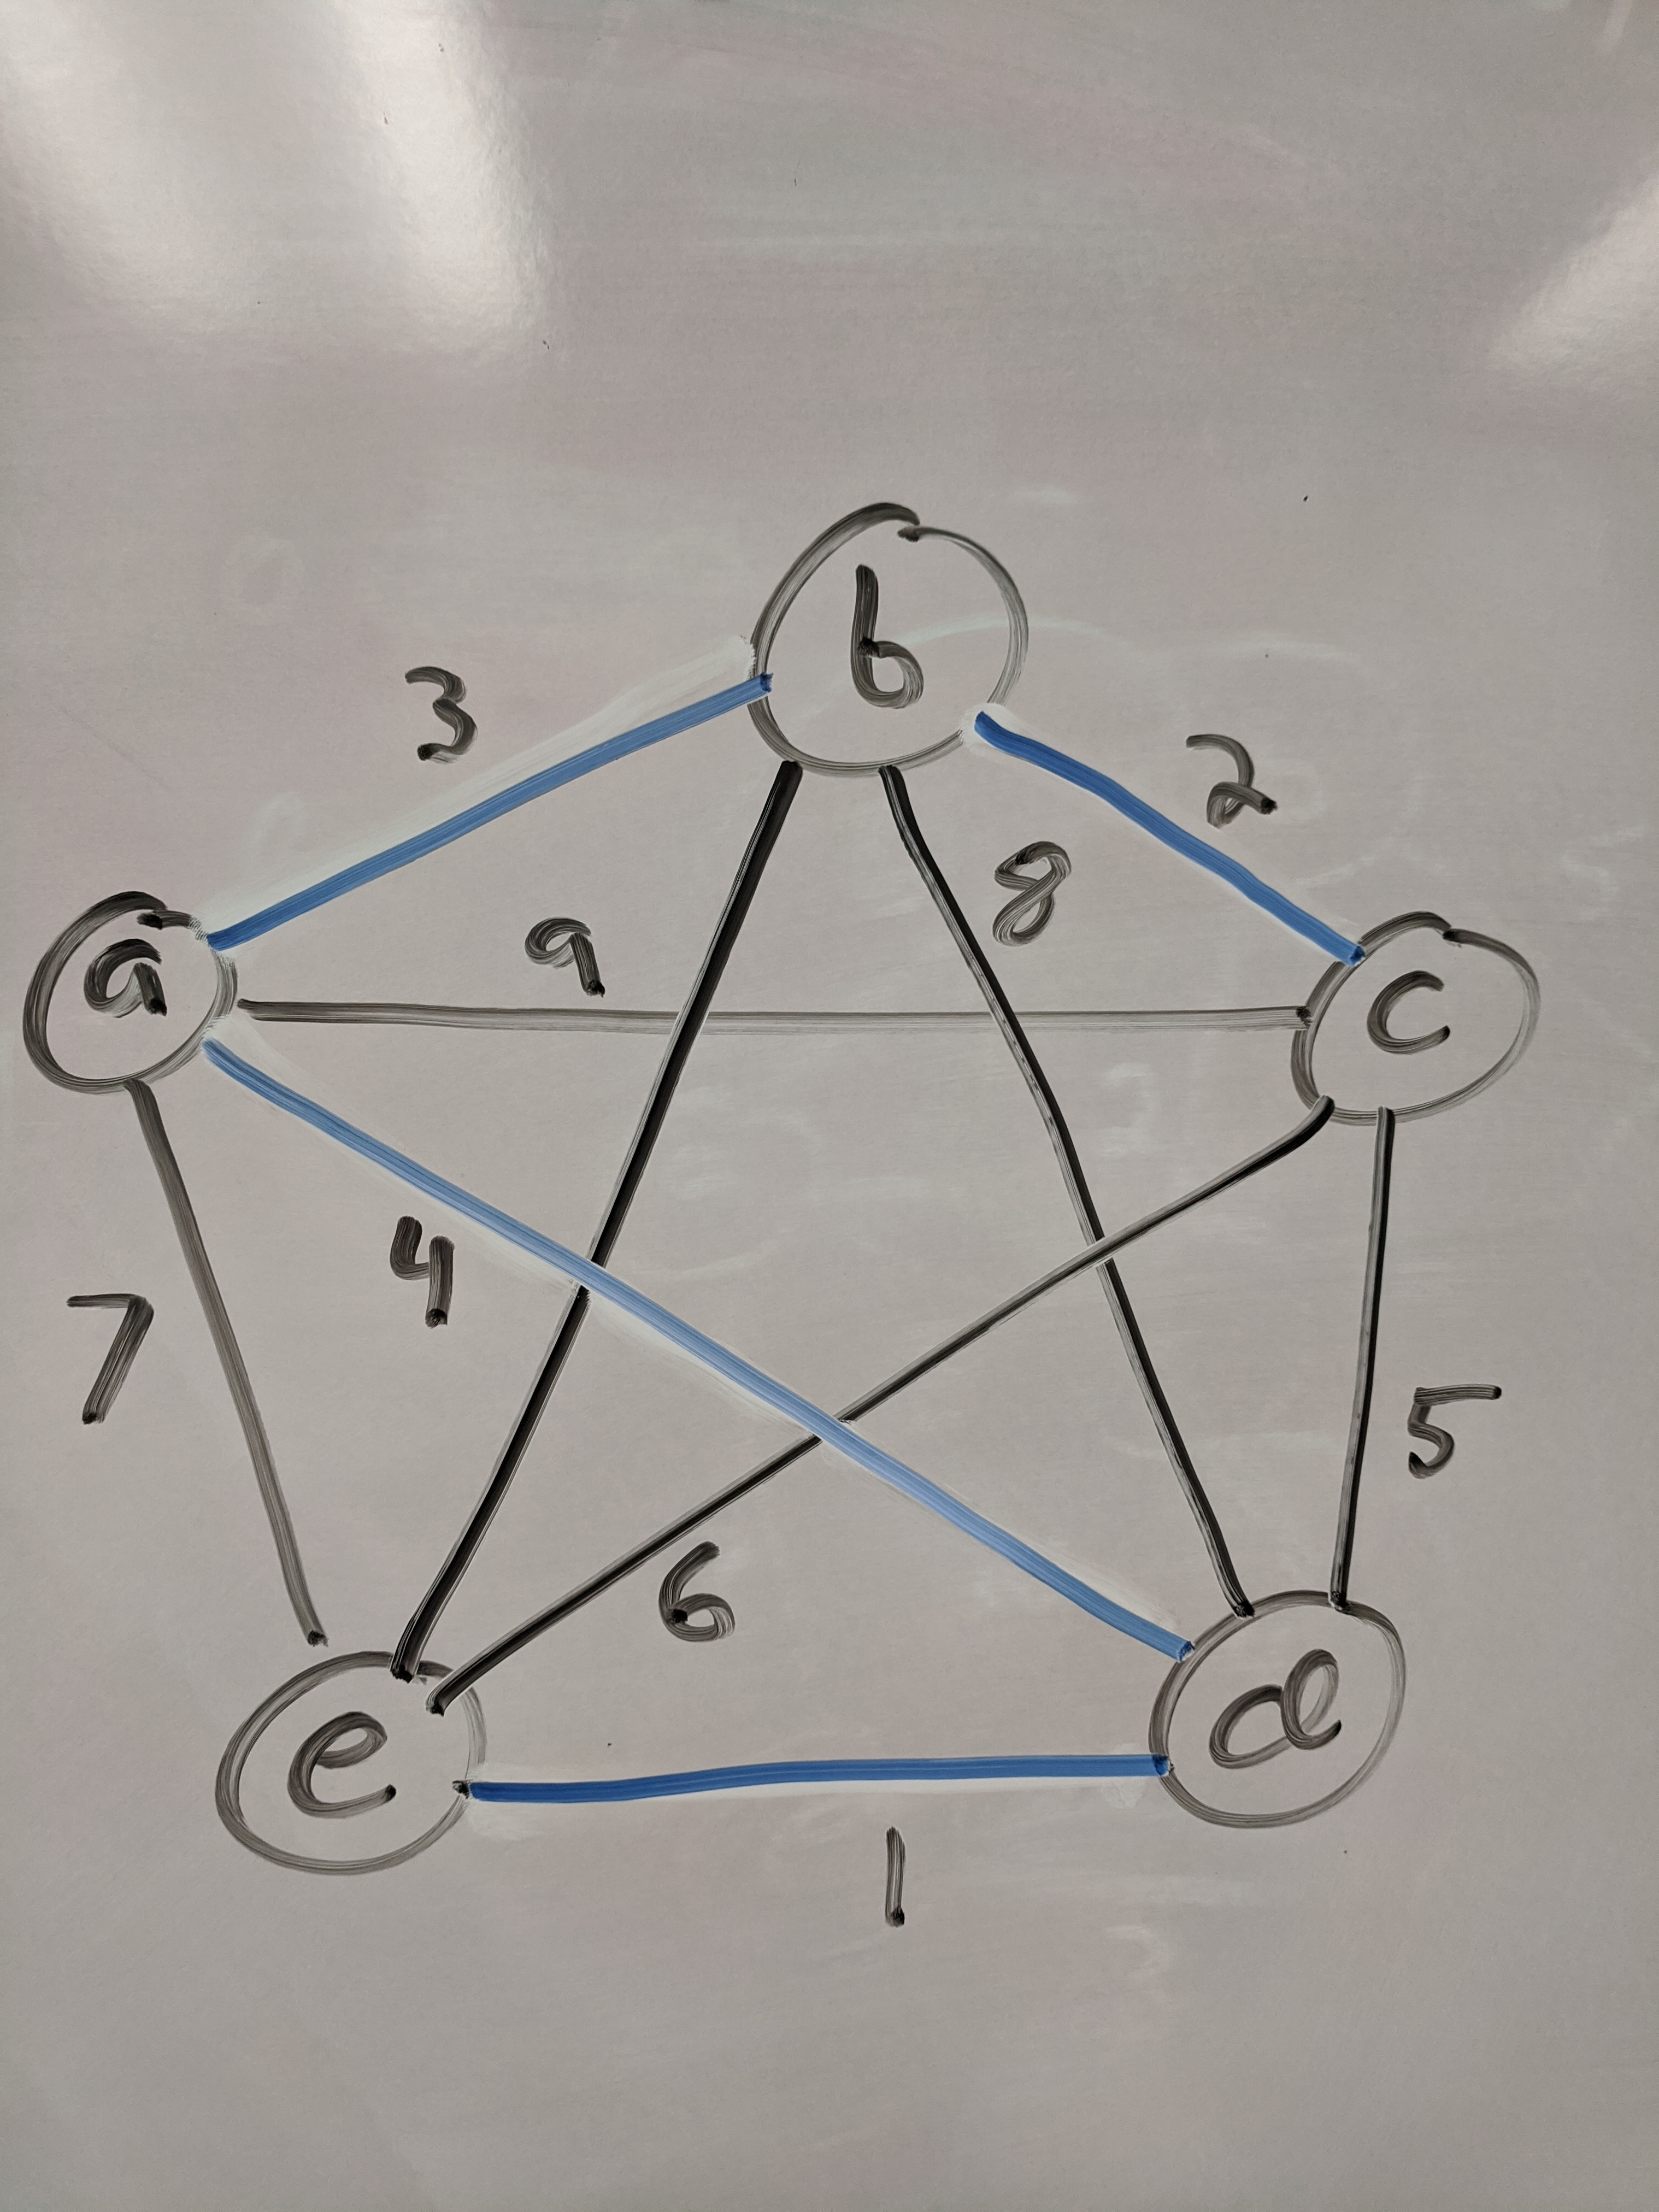
\includegraphics[height=160pt]{13-tspti-mst.jpg}
  \end{center}
\end{frame}

\begin{frame} \frametitle{Approximate TSPTI: Preorder Traversal}
  \begin{center}
    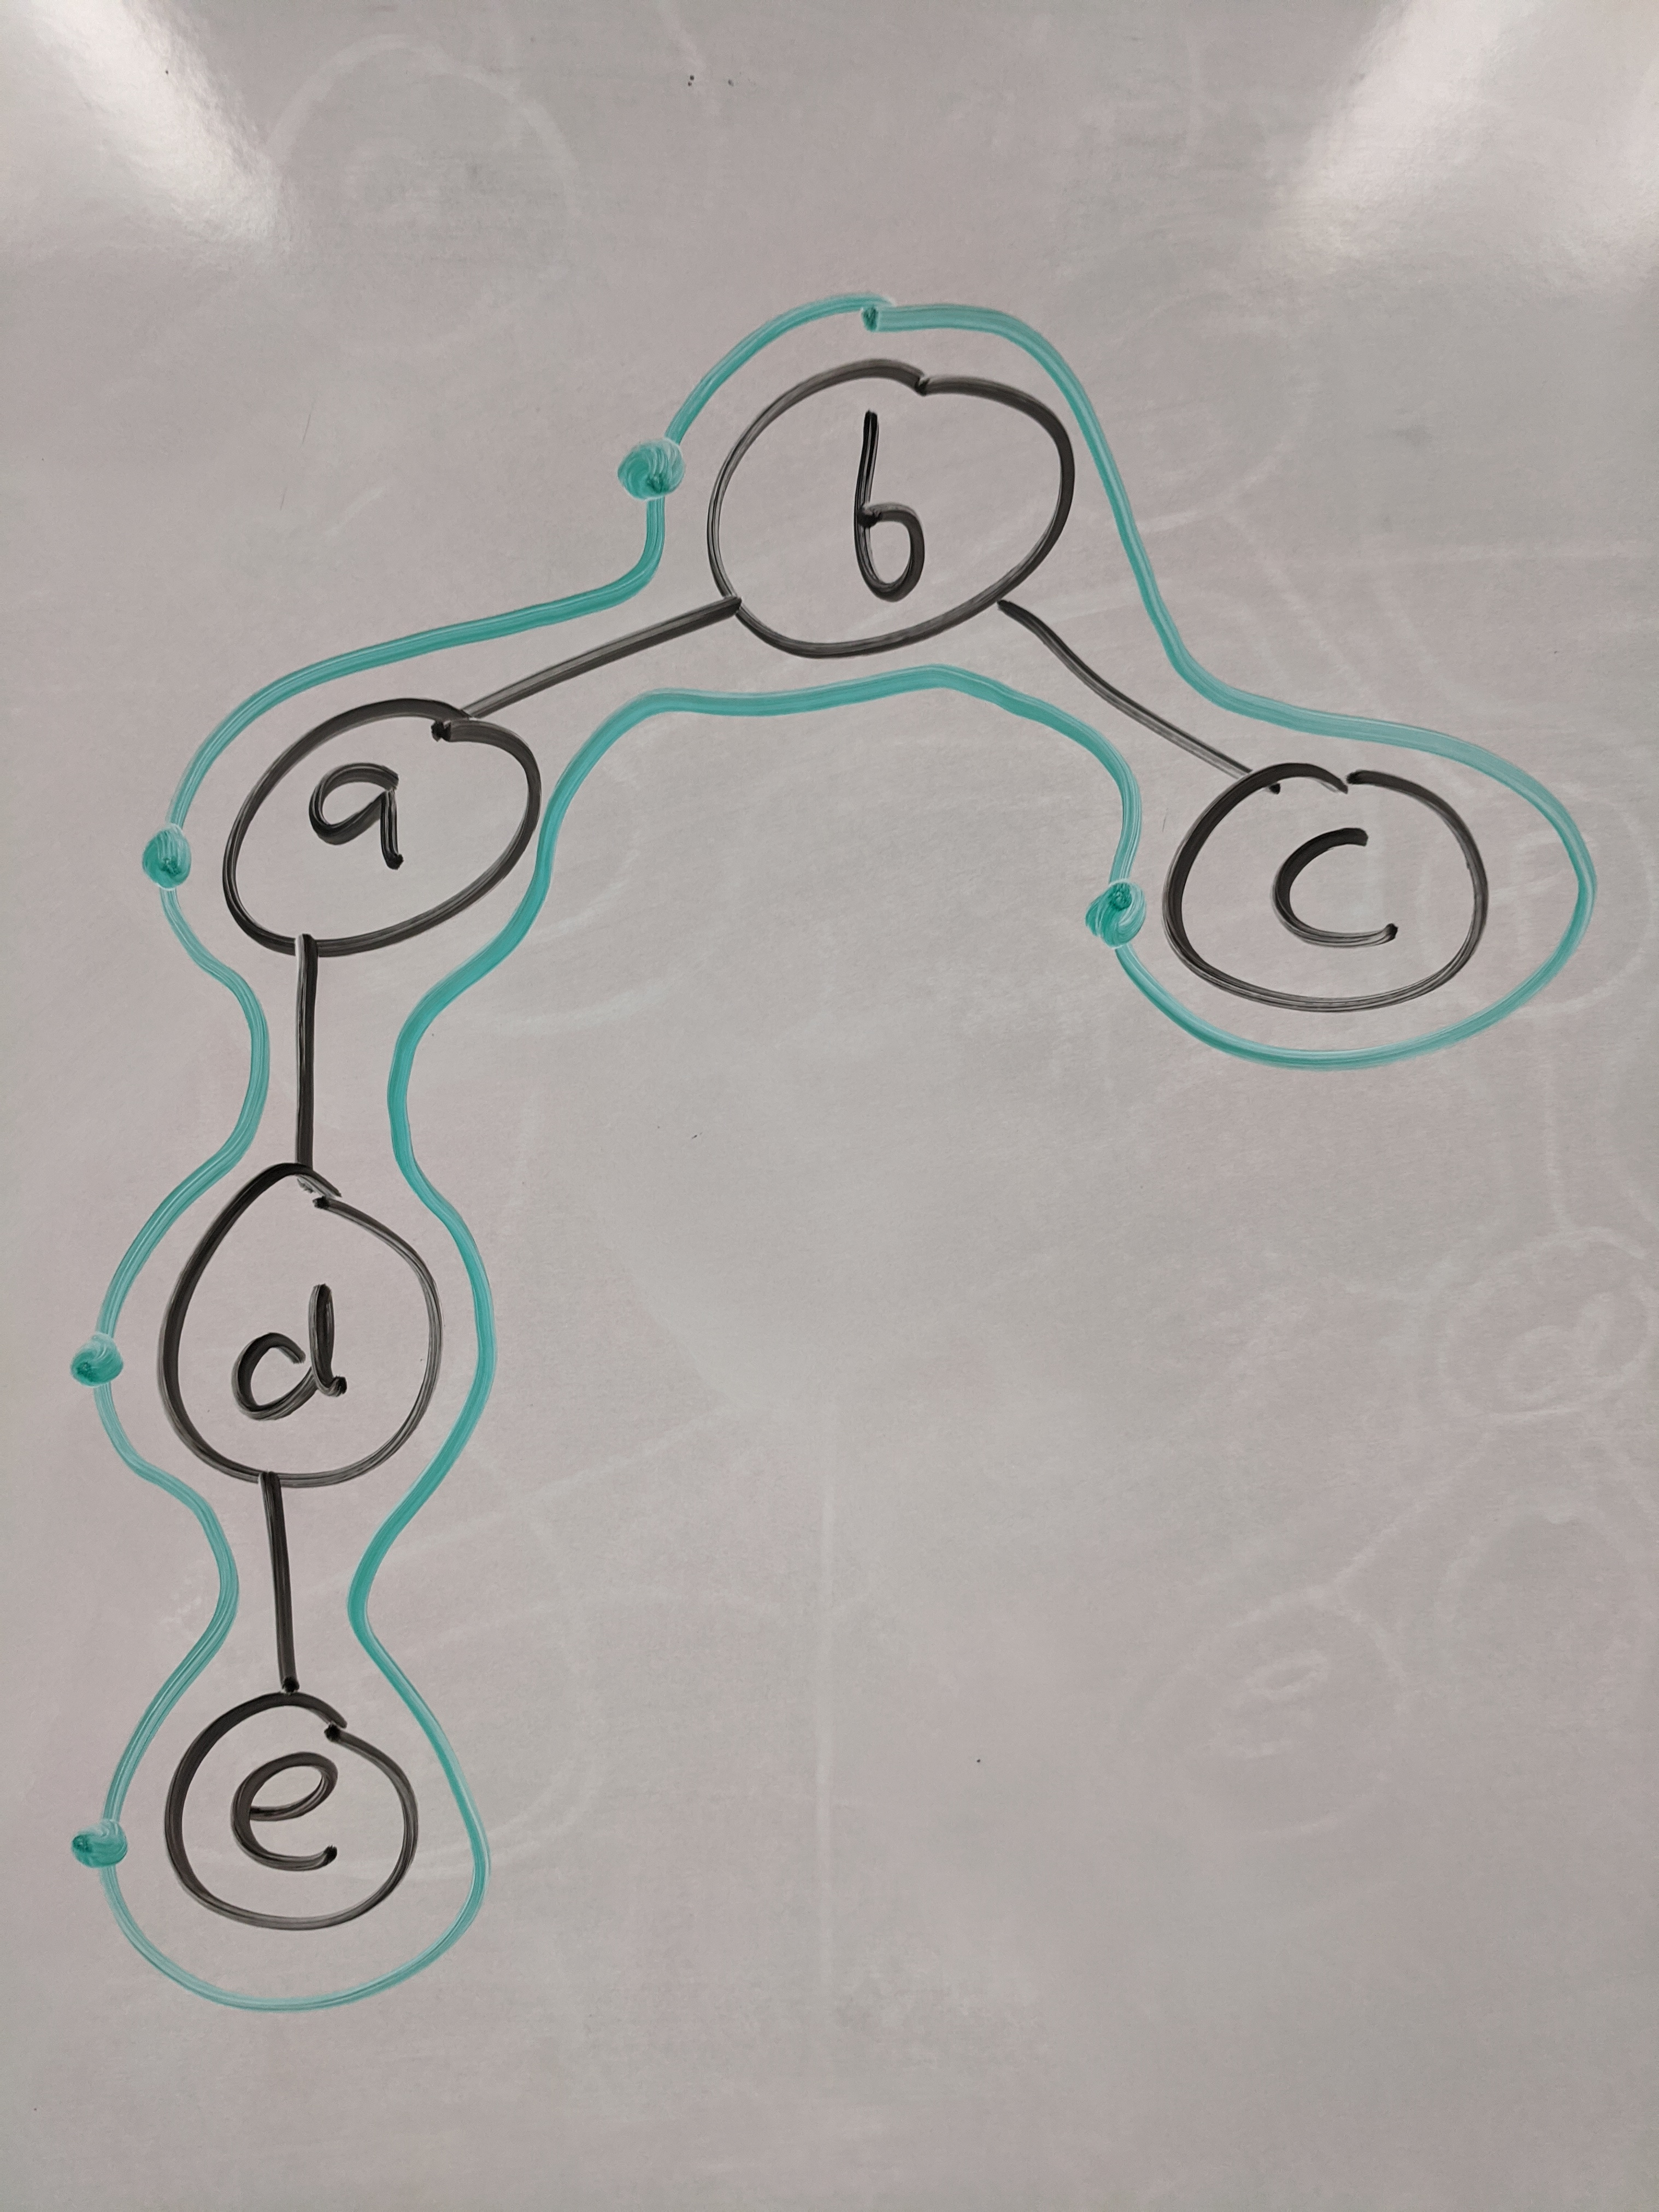
\includegraphics[height=160pt]{13-tspti-preorder.jpg}
  \end{center}
\end{frame}

\begin{frame} \frametitle{Approximate TSPTI: Solution}
  \begin{center}
    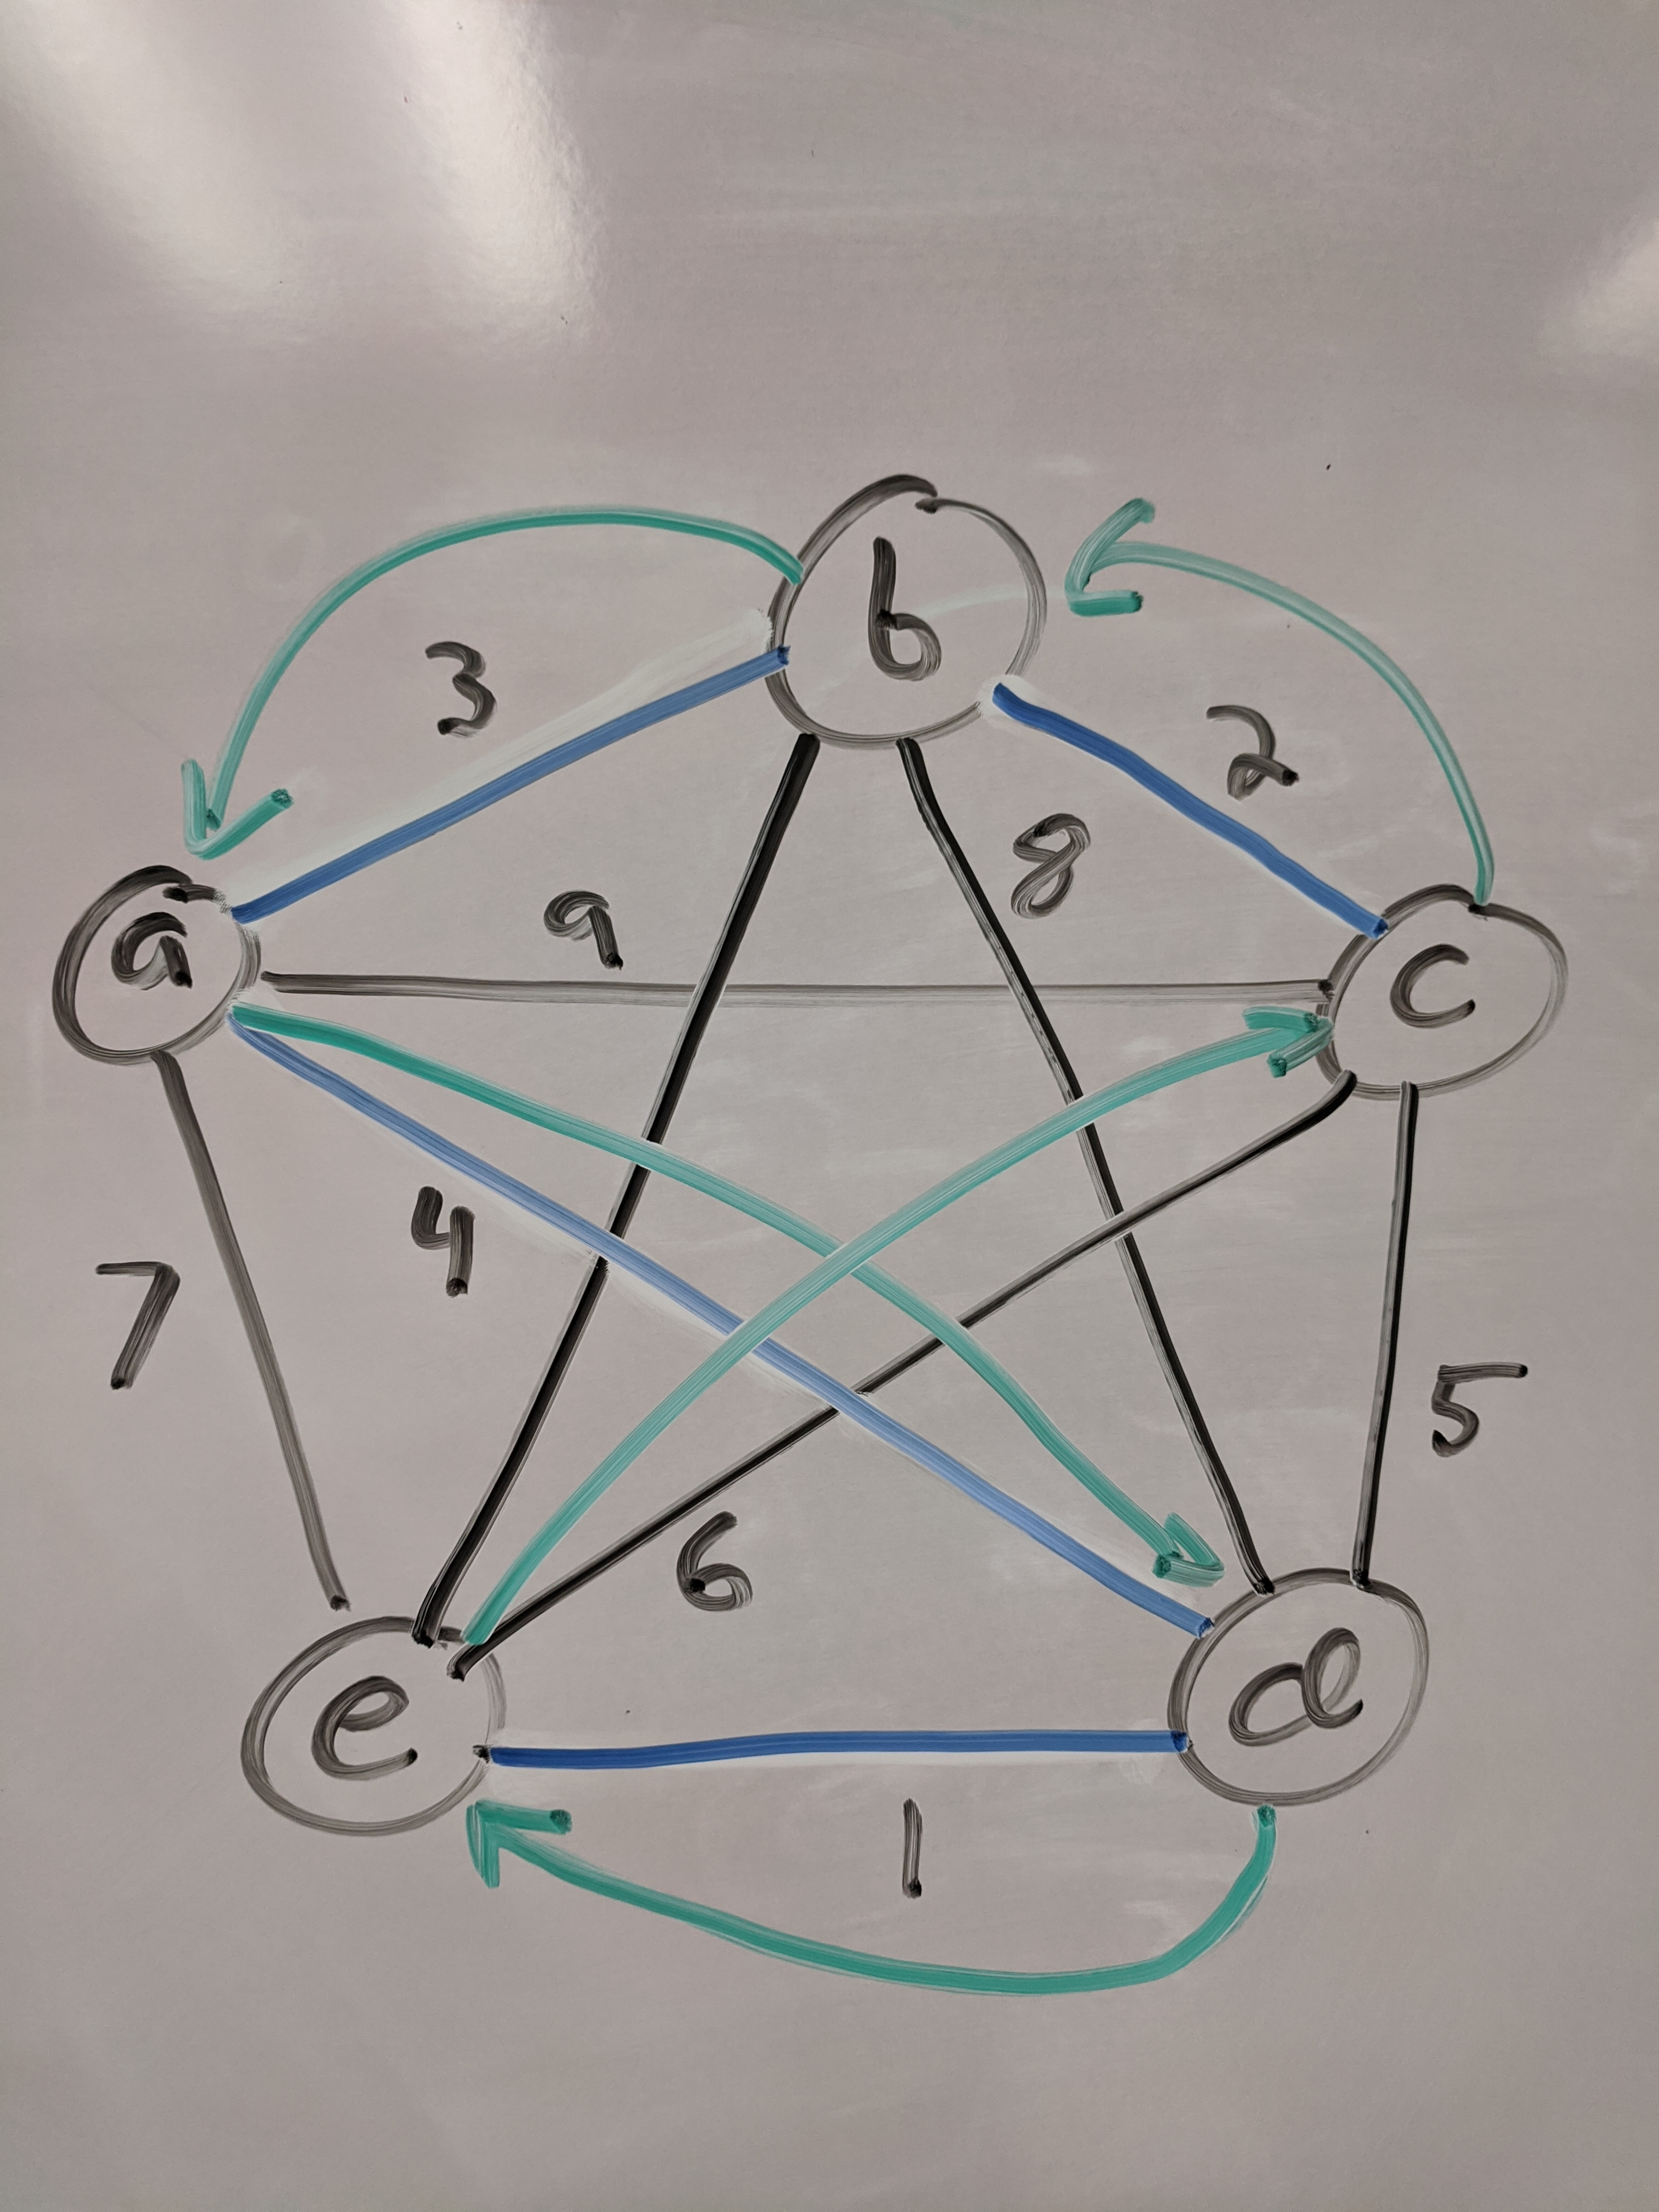
\includegraphics[height=160pt]{13-tspti-output.jpg}
  \end{center}
\end{frame}

\begin{frame} \frametitle{TSPTI Performance}
\textbf{Lemma}: APPROX-TSPTI is a 2-approximation algorithm \\
\textbf{Proof Sketch}:
\begin{itemize}
  \item let $H^\star$ be an optimal Hamiltonian cycle for $G$
  \item (1) every spanning tree is one edge short of a cycle; and weights are nonnegative;
    so the weight of our tree $T$ obeys $w(T) \leq w(H^\star)$
  \item (2) a \emph{full tour} $W$ is the sequence of vertices in both a preorder and postorder
    tour, and has weight $w(W) = 2 w(T)$
  \item (3) combining (1) and (2), $w(W) \leq 2 w(H^\star)$
  \item (4) our $H$ is like $W$ with some vertices removed, so $w(H) \leq w(W)$
  \item combining (3) and (4),
    \[ w(H) \leq w(W) \leq 2 w(H^\star) \]
\end{itemize}
\end{frame}

\begin{frame} \frametitle{Summary}
Vertex cover:
\begin{itemize}
  \item NP-complete
  \item exact exhaustive search alg. takes $\Theta(2^n m)$ time
  \item 2-approximate alg. takes $\Theta(n+m)$ time \stanza
\end{itemize}

TSP:
\begin{itemize}
  \item NP-complete
  \item exact exhaustive search alg. takes $\Theta(n!)$ or $\Theta(2^m(n+m))$ time
  \item 2-approximate algorithm takes $O(m + n \log n)$ time
\end{itemize}
\end{frame}

\end{document}
